\chapter{Analyse du taux de réussite au bac}

\section{Introduction}

Ce chapitre est consacré à l’analyse du taux de réussite au baccalauréat au Sénégal sur la période 2006–2024. 
L’objectif est de mettre en lumière les tendances globales et spécifiques aux séries concernées par les réformes, à travers une exploration visuelle des données.

Nous débuterons par l’évolution du nombre d’inscrits et du taux de réussite global, avant de nous concentrer sur les séries spécifiques analysées dans ce travail, notamment les séries arabes, franco-arabes, STEG, G. 

Des visualisations comparatives permettront d’identifier les ruptures, dynamiques et écarts entre les différentes filières. 
En complément, une modélisation prédictive sera réalisée afin d’estimer l’évolution théorique du taux de réussite en l’absence des réformes, offrant ainsi une base de comparaison pour mesurer leur impact.

\section{Analyse de globale}

\newpage
\subsection{Évolution des effectifs}

\begin{figure}[ht]
\centering
\caption{Évolution du nombre d'inscrits, présents et admis au bac (2006-2024)}
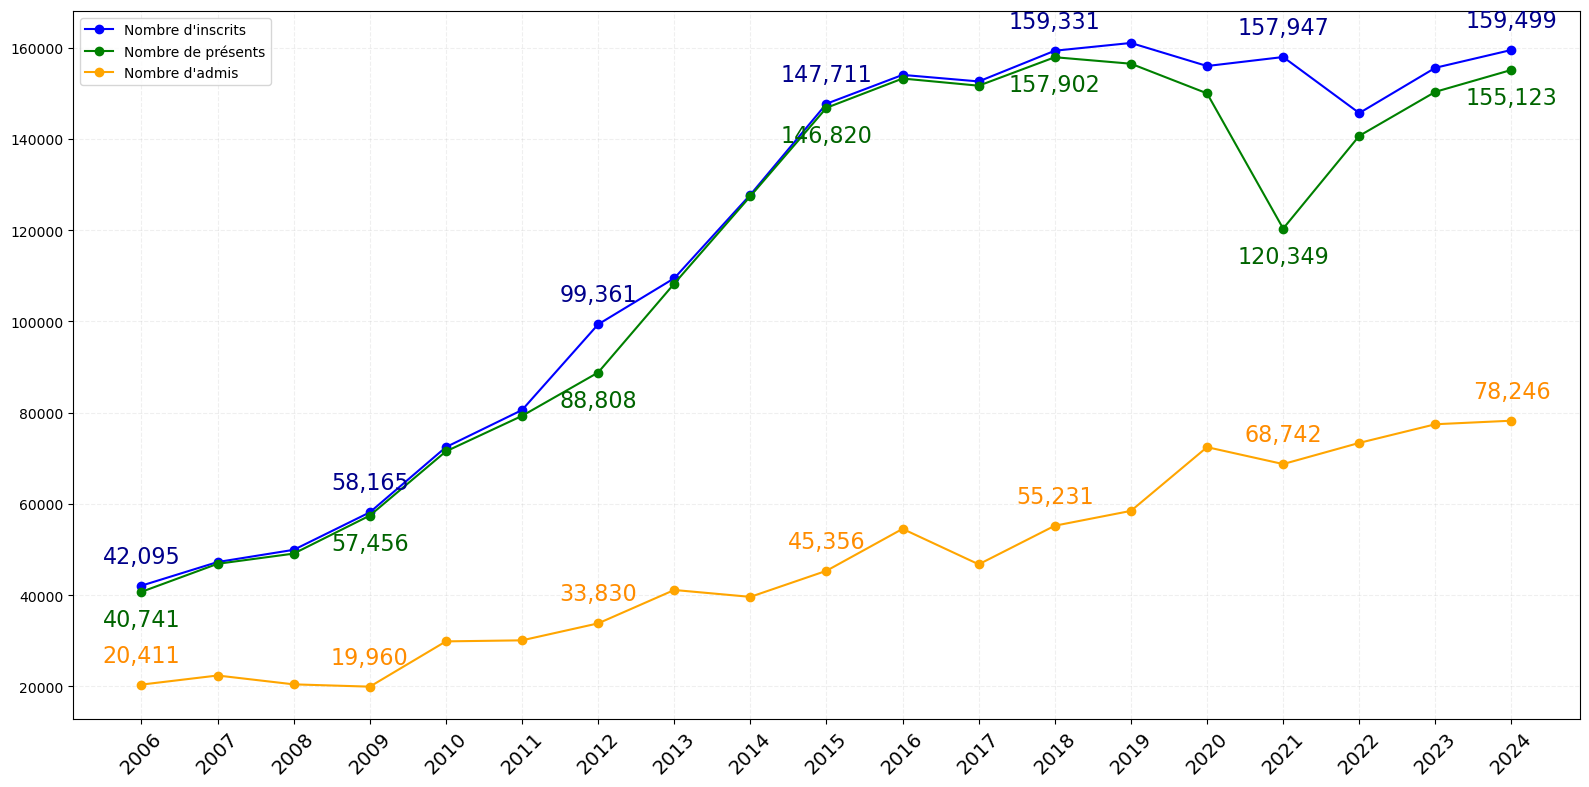
\includegraphics[width=1\textwidth]{figure/Inscrits_bac.png}
\label{fig:inscrits_admis}
\end{figure}

La figure (Figure~\ref{fig:inscrits_admis}) représente l’évolution du nombre d’inscrits, de présents et d’admis au baccalauréat entre 2006 et 2024. 
L’observation met en évidence deux phases temporelles distinctes.

\textbf{Phase 1 — Croissance rapide (2006–2015)}  

Durant cette période, le système éducatif sénégalais connaît une expansion notable du nombre de candidats au bac. 
Le nombre d’inscrits passe de 42 095 en 2006 à 147 711 en 2015, soit une croissance d’environ \textbf{250\,\%} en 9 ans.

Les admis augmentent également mais de manière moins rapide, passant de 20 411 en 2006 à 45 356 en 2015, soit une hausse d’environ \textbf{125\,\%}. 
Ce décalage entre l’augmentation des présents et celle des admis révèle un déséquilibre croissant sur les performances au baccalauréat.

\textbf{Phase 2 — Stabilisation relative (2015–2024)}  

À partir de 2015, le nombre d’inscrits se stabilise autour de 150 000 à 160 000 candidats par an. 
La croissance ralentit, marquant une saturation ou une stabilisation des flux en fin de cycle secondaire. 
Une chute brutale du nombre de présents est toutefois observée en 2021, ce qui peut être associé aux perturbations causées par la pandémie de COVID-19.

Les admissions au baccalauréat continuent d'afficher une croissance modérée, atteignant 78 246 en 2024. Toutefois, cette évolution reste notablement faible comparée au nombre de candidats inscrits et présents.

\subsection{Évolution du taux de réussite}

\begin{figure}[ht]
\centering
\caption{Évolution du taux de réussite au bac (2006-2024)}
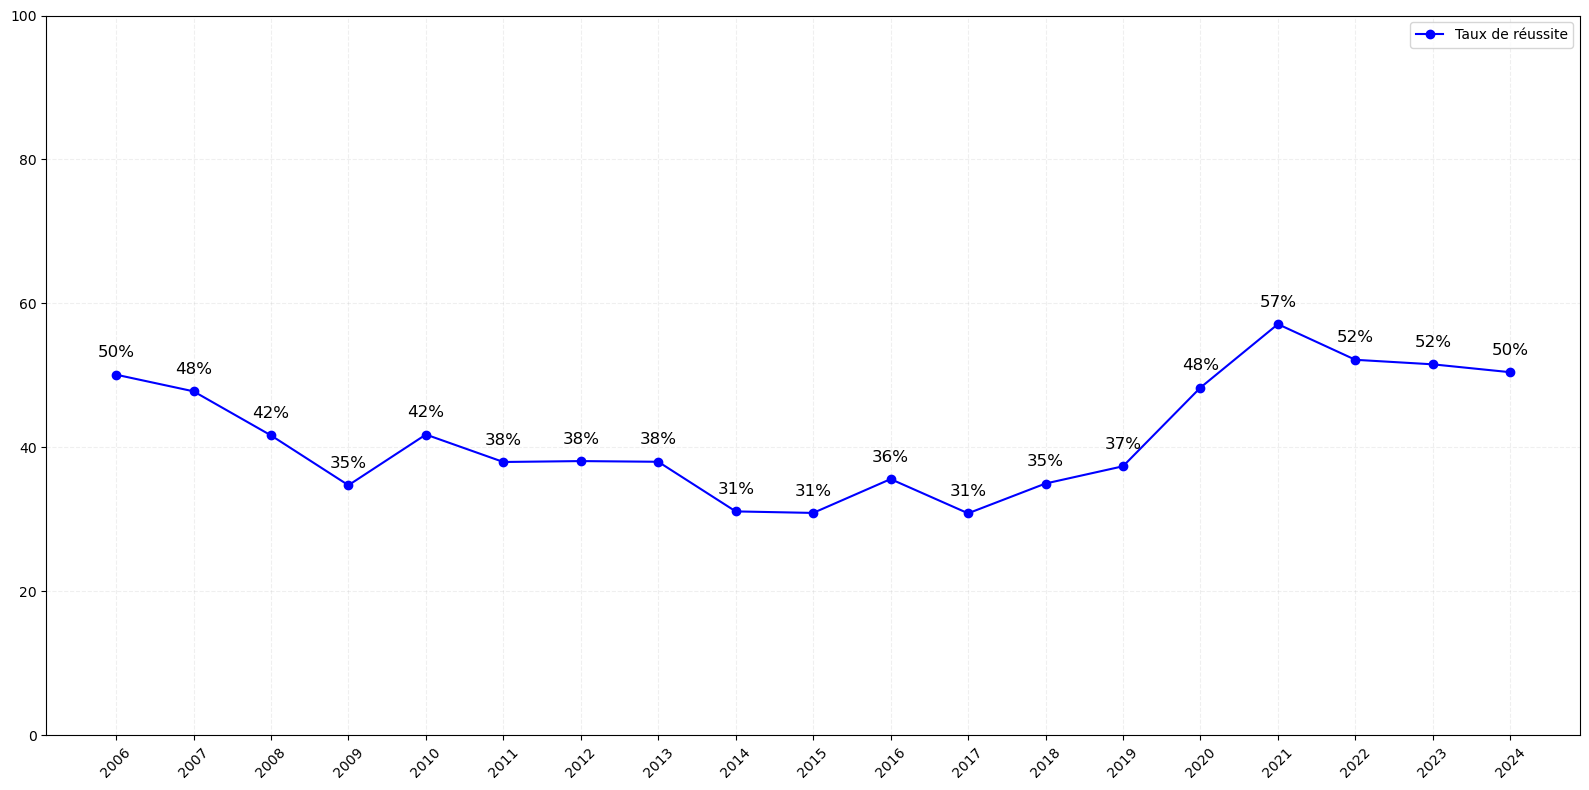
\includegraphics[width=1\textwidth]{figure/taux_bac.png}
\label{fig:taux_reussite}
\end{figure}

La figure (Figure~\ref{fig:taux_reussite}) illustre l’évolution du taux de réussite au baccalauréat sénégalais entre 2006 et 2024. 
L’analyse révèle des fluctuations marquées, avec des périodes de déclin et de reprise.


\textbf{Période 2006–2017 — Baisse significative}

Durant cette phase, le taux de réussite connaît une chute alarmante, passant de 50\% en 2006 à 31\% en 2017. 
Cette diminution de près de 20 points en onze ans souligne des difficultés structurelles.

\textbf{Période 2017–2024 — Progression notable}

À partir de 2017, le taux de réussite montre une nette amélioration, atteignant 50\% en 202, avec un pic record 57\% en 2021(ce taux élevé peut s'expliquer par la chute brutale du nombre de présents liée à la pandémie, puisqu'il est calculé en fonction des candidats ayant effectivement passé l’examen). 
Toutefois, une légère baisse est observée entre 2021 et 2024, ce qui peut être source d’inquiétude.

\bigskip

Malgré une légère amélioration récente, le taux de réussite au baccalauréat demeure généralement trop faible pour un système éducatif aspirant à la performance.

\newpage
\section{Analyse de la transition entre les séries G et STEG}

La réforme du baccalauréat technique au Sénégal, concrétisée par le décret de 2019, marque un tournant important dans l’organisation de la série Techniques quantitatives d’économie et de gestion.
Elle prévoit \textbf{la suppression progressive de la série G}, au profit de la nouvelle série \textbf{STEG}.
Cette dernière vise à mieux articuler les enseignements généraux et technologiques afin de développer chez les élèves des compétences applicables dans l’enseignement supérieur et la vie professionnelle.

Conformément au décret, la série G a continué à être organisée jusqu’en 2022, date de sa dernière session. À partir de 2023, seule la série STEG est maintenue. 
Cette transition permet d’évaluer les effets de la réforme en comparant les performances (nombre d’inscrits et taux de réussite) de la série STEG à celles de son prédécesseur, la série G.

\subsection{Évolution du nombre d'inscrits dans les séries G et STEG}

\begin{figure}[ht]
\centering
\caption{Évolution du nombre d'inscrits dans les séries G et STEG (2006-2024)}
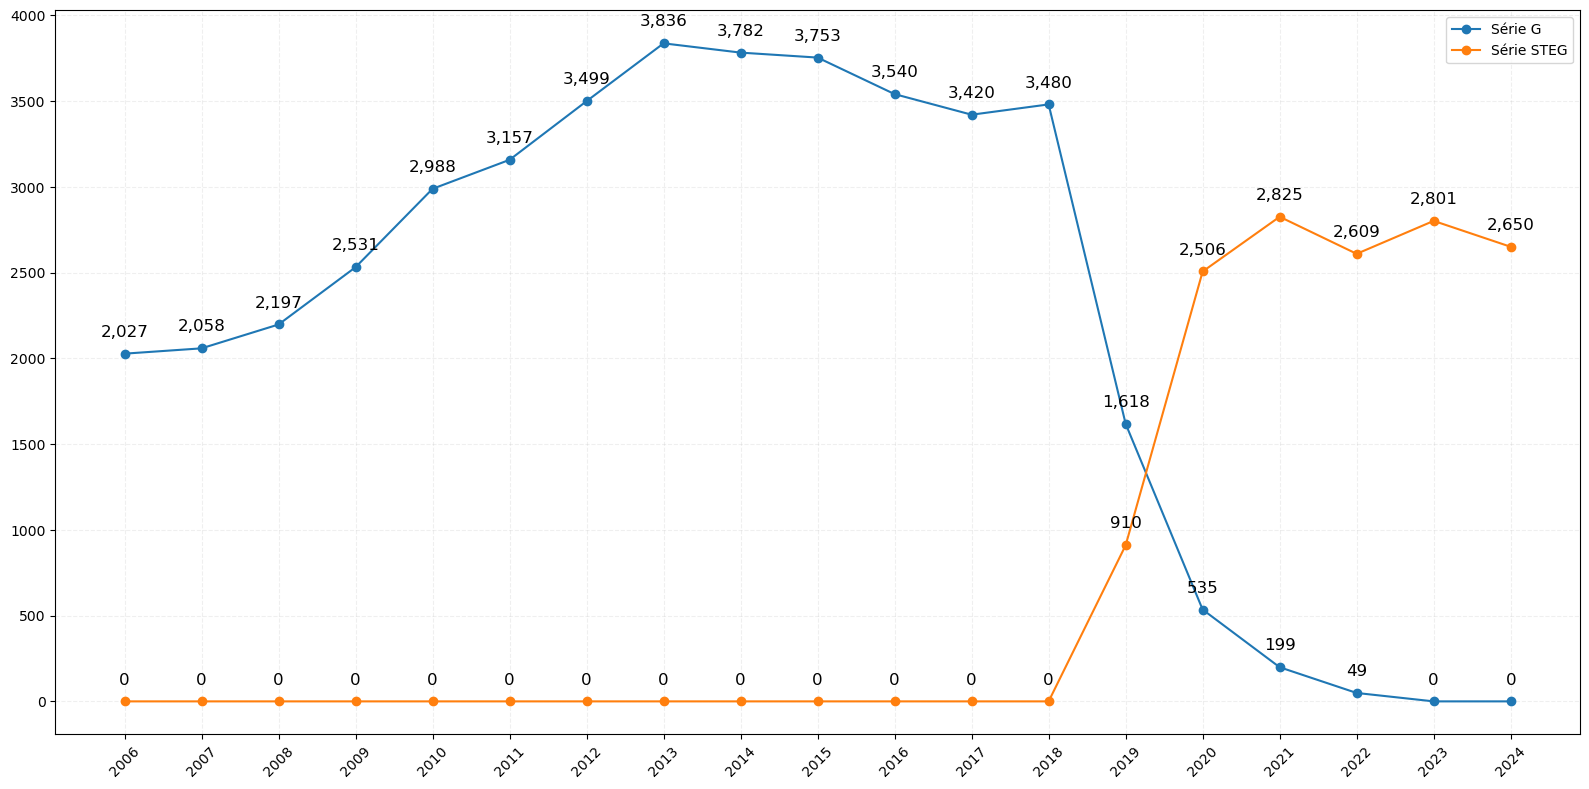
\includegraphics[width=1\textwidth]{figure/Inscrits_bac_STEG.png}
\label{fig:inscrits_STEG}
\end{figure}

La figure (Figure~\ref{fig:inscrits_STEG}) montre l’évolution du nombre d’inscrits au baccalauréat dans les séries G et STEG entre 2006 et 2024. 

Jusqu’en 2018, seule la série G est présente, avec un pic d’inscription atteint entre 2012 et 2014. À partir de 2019, la série STEG est introduite et connaît une croissance rapide, tandis que les effectifs de la série G diminuent progressivement, jusqu’à leur extinction en 2023.

Ce croisement entre les deux courbes montre clairement une transition bien gérée sur le plan quantitatif, avec un transfert progressif des effectifs. 
Dès 2020, les inscriptions en STEG dépassent celles de la série G, traduisant une bonne adhésion des établissements et des élèves à la réforme.

\subsection{Évolution du taux de réussite dans les séries G et STEG}

\begin{figure}[ht]
\centering
\caption{Évolution du taux de réussite dans les séries G et STEG (2006-2024)}
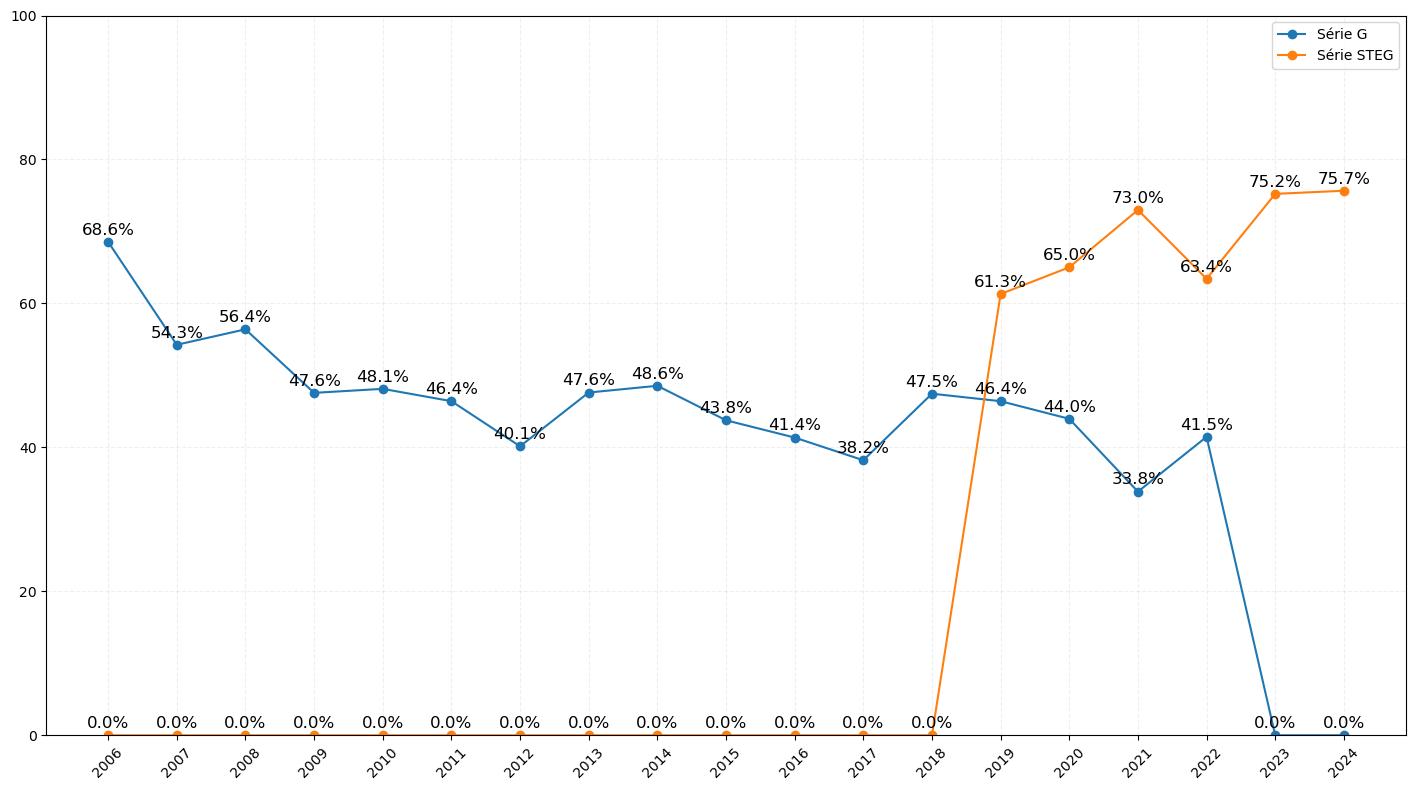
\includegraphics[width=1\textwidth]{figure/taux_bac_STEG.png}
\label{fig:taux_reussite_STEG}
\end{figure}

La figure (Figure~\ref{fig:taux_reussite_STEG}) met en perspective les performances des deux séries en termes de réussite. 
On observe une forte variabilité du taux de réussite en série G, fluctuant généralement entre \textbf{40\%} et \textbf{50\%}, avec une tendance légèrement décroissante.

En revanche, la série STEG, dès sa première session en 2019, affiche \textbf{des taux de réussite supérieurs}, allant de \textbf{60\%} à plus de \textbf{75\% en 2024}.
Ce résultat semble valider l’objectif de la réforme qui est de renforcer l'efficacité du système en recentrant les contenus pédagogiques autour de compétences concrètes, professionnelles et transversales.

\bigskip

En somme, \textbf{la série STEG se distingue par de meilleures performances en matière de réussite}, tout en parvenant à capter un volume d’élèves au moins équivalent, voire supérieur, à celui de la série G à son apogée. 
Cela confirme la pertinence de la réforme dans le contexte de modernisation du système éducatif sénégalais.

\newpage
\section{analyse des séries Arabes et Franco-Arabes}

Le système éducatif sénégalais a progressivement intégré l'enseignement de l'arabe dans le secondaire, avec la création de séries Franco-arabes en 2000.
Cependant, face à la prolifération des établissements d'enseignement exclusivement arabe et des instituts islamiques, le décret n°2013-057 a modifié et complété ces dispositions a fin de mieux répondre à la demande sociale suivantes: 
\begin{itemize}
    \item Littératures et Civilisations arabes (L-AR)
    \item Mathématiques et Sciences physiques (S1-AR)
    \item Sciences expérimentales (S2-AR)
\end{itemize}

Les études secondaires arabes sont désormais sanctionnées par des diplômes appelés \textbf{baccalauréats arabes}, tandis que les enseignements bilingues franco-arabe donnent lieu à des \textbf{baccalauréats franco-arabes}.
\subsection{Série LA et LAR}

\begin{figure}[ht]
\centering
\caption{Évolution du nombre d'inscrits et du taux de réussite dans les séries LA et LAR (2006-2024)}
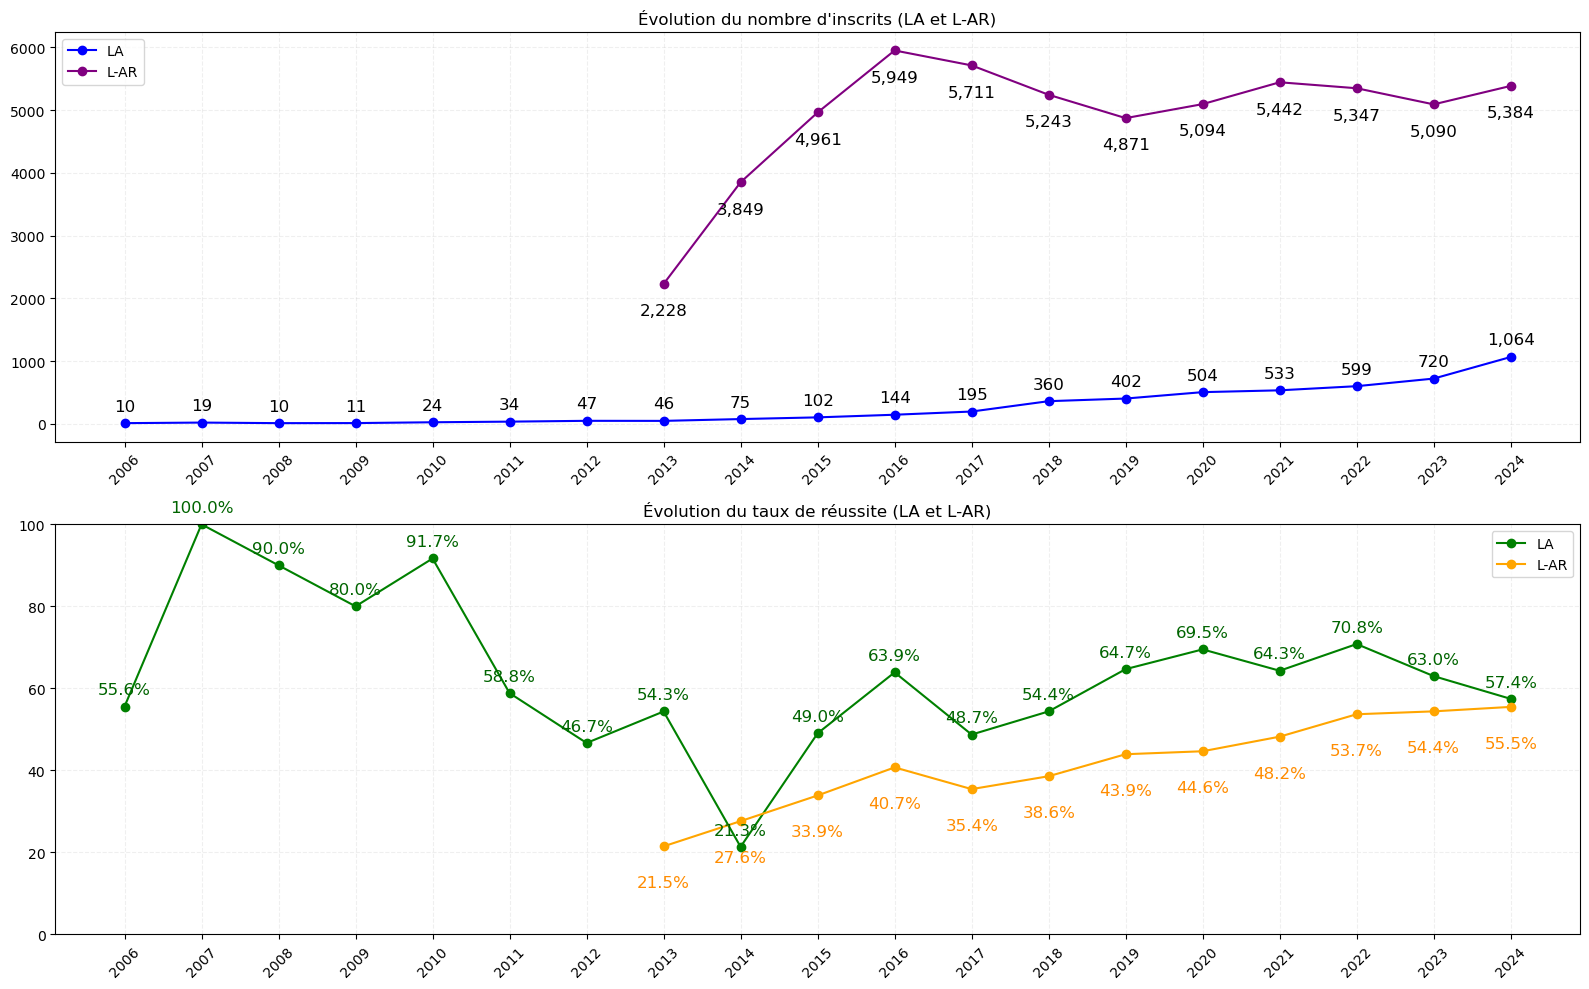
\includegraphics[width=1\textwidth]{figure/bac_LA_LAR.png}
\label{fig:LA_LAR}
\end{figure}

La Figure \ref{fig:LA_LAR} illustre l'évolution du nombre d'inscrits et des taux de réussite aux baccalauréats des séries Littératures et Sciences sociale (franco-arabe) LA et Littératures et Civilisations Arabes (L-AR) entre 2006 et 2024.

\subsubsection{Évolution du nombre d'inscrits}

La série LA, présente depuis 2000, a toujours eu un nombre d'inscrits relativement faible avec une légère croissance, passant de 10 en 2006 à 1 064 en 2024.  
Cette augmentation, bien que modérée, témoigne d'un intérêt croissant et soutenu pour cette filière au fil des ans.

En revanche, la série L-AR, introduite en 2013, a connu une croissance fulgurante dès son apparition. 
Elle a attiré 2 849 inscrits en 2013, atteignant un pic de 5 949 en 2015. Bien qu'une légère diminution ait été observée par la suite, le nombre d'inscrits en L-AR s'est stabilisé autour de 5 000 à 5 300, avec 5 184 inscrits en 2024. 
La série L-AR a rapidement dominé en termes d'effectifs, surpassant de loin la série LA, ce qui suggère une forte adhésion à cette nouvelle filière et un transfert significatif des étudiants vers cette option réformée.

Cette dynamique met en évidence la réussite de la mise en place du baccalauréat arabe, notamment la série L-AR, qui a su capter un volume important d'étudiants, répondant ainsi à la demande sociale et aux objectifs de structuration des études arabes au Sénégal.

\subsubsection{Évolution du taux de réussite}

La série LA a montré une grande variabilité de ses taux de réussite. Après un début à 55,6\% en 2006, elle a connu des pics remarquables à 90\% en 2008 et 91,7\% en 2010, des chiffres à juger avec prudence car l’effectif était considérablement faible, avec une moyenne d’environ 15 candidats entre 2006 et 2010.
Cependant, des baisses significatives ont suivi, avec des taux chutant à 46.7\% en 2012 et un point bas à 27.5\% en 2013. 
Par la suite, le taux de réussite en LA a montré une tendance à la reprise, atteignant 63.9\% en 2015 avant de se stabiliser autour de 50\% à 70\% dans les années suivantes, pour finir à 57.4\% en 2024. 

En comparaison, la série L-AR, bien que plus récente, a affiché des taux de réussite plus cohérents (explicables par un nombre de candidats assez élevé) avec une tendance croissante. 
À son introduction en 2013, le taux de réussite était d'environ 21\%, montant progressivement pour atteindre 55.5\% en 2024 qui se rapproche de celui de la série LA.
Ce résultat est d'autant plus notable que la série L-AR a géré un volume d'inscrits considérablement plus important.

En conclusion, la série L-AR, malgré un volume d'effectifs beaucoup plus important, a globalement réussi à maintenir des taux de réussite compétitifs et plus stables que ceux de la série LA.
Cette performance suggère que la réforme ayant introduit la série L-AR, avec son nouveau référentiel et ses objectifs d'harmonisation, a contribué à une meilleure efficacité du système pour les filières arabes au Sénégal.

\subsection{Série S2A}

\begin{figure}[ht]
\centering
\caption{Évolution du nombre d'inscrits et du taux de réussite dans la série S2A (2006-2024)}
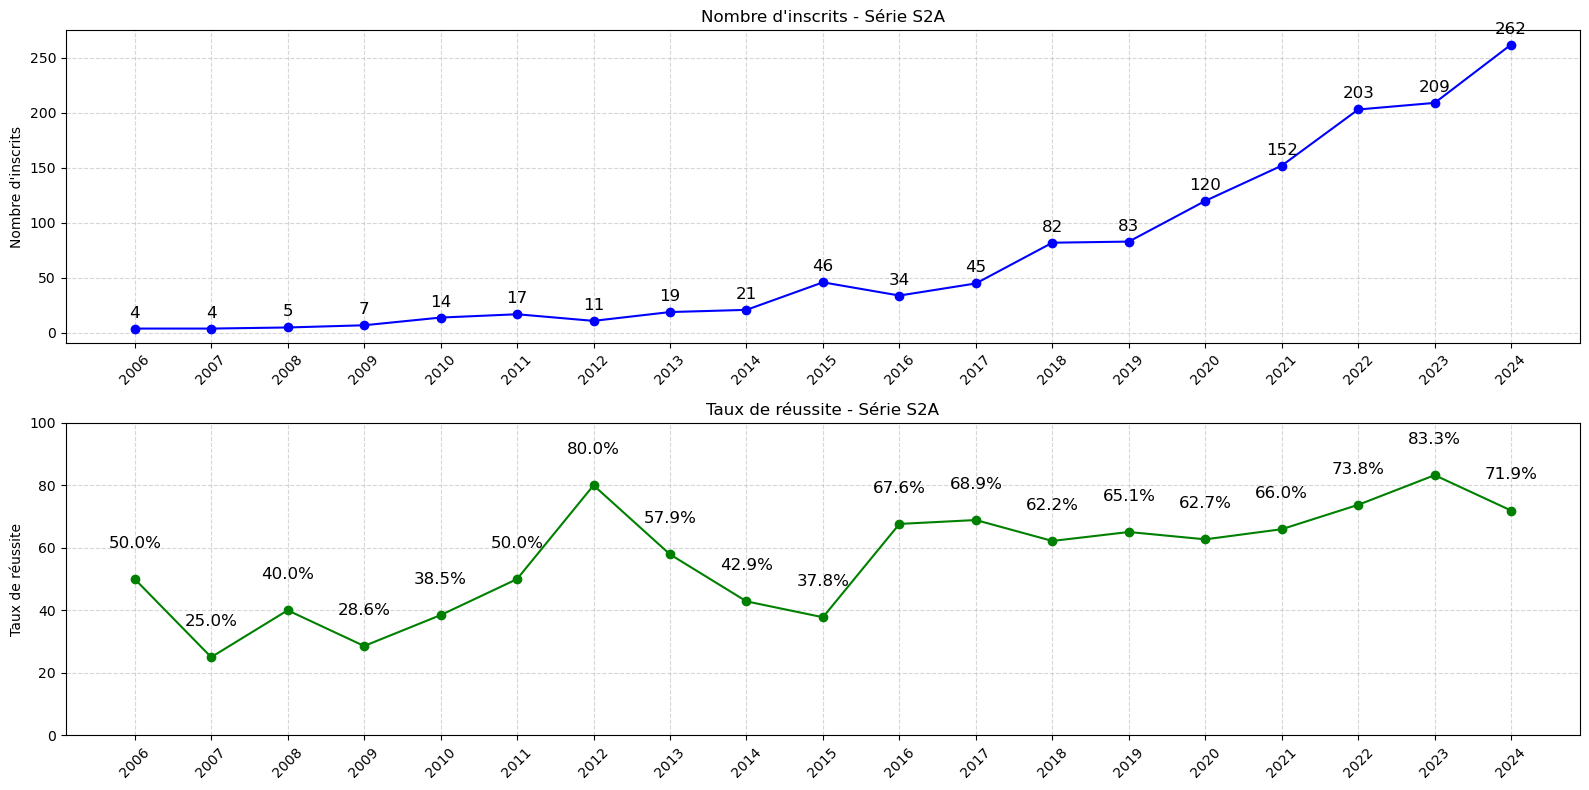
\includegraphics[width=1\textwidth]{figure/bac_S2A.png}
\label{fig:S2A}
\end{figure}

La figure (Figure~\ref{fig:S2A}) montre l'évolution du nombre d'inscrits et du taux de réussite dans la série Sciences appliquées (S2A).

\subsubsection{Évolution du nombre d'inscrits}
De 2006 à 2016, la série S2A a connu une première phase de faible adhésion, avec une légère tendance à la hausse, passant de 4 inscrits en 2006 à 34 en 2016.
À partir de 2017, la série S2A enregistre une croissance exponentielle de ses effectifs, atteignant 262 inscrits en 2024.
La série parvient ainsi à capter un volume d’élèves en nette progression, traduisant une reconnaissance croissante de son importance.

\subsubsection{Évolution du taux de réussite :}
Concernant le taux de réussite, la série S2A présente une forte variabilité au début de la période, en raison du faible nombre de candidats. Après un taux de 50\% en 2006, il chute à 25\% en 2007, puis atteint un pic exceptionnel de 80\% en 2011.
À partir de 2016, on observe une nette amélioration, avec des taux de réussite généralement supérieurs à 60\%. La série atteint même 83,3\% en 2023, avant de légèrement reculer à 71,9\% en 2024.

\bigskip

Malgré des débuts irréguliers, la série S2A affiche de bonnes performances sur la dernière décennie, confirmant son potentiel de réussite croissant.

\subsection{Série S1A}

\begin{figure}[ht]
\centering
\caption{Évolution du nombre d'inscrits et du taux de réussite dans la série S2A (2006-2024)}
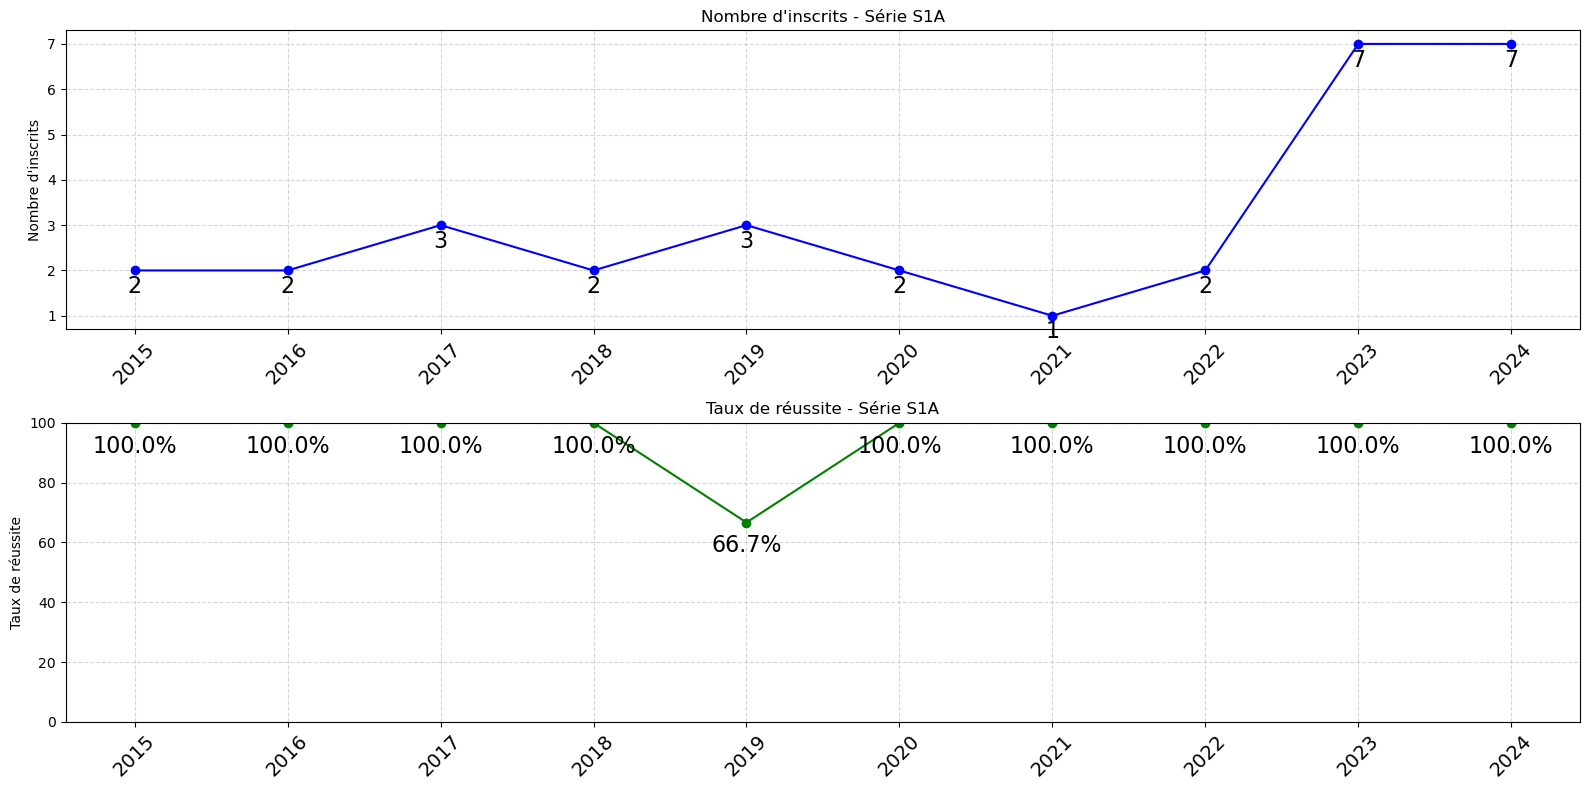
\includegraphics[width=1\textwidth]{figure/bac_S1A.png}
\label{fig:S1A}
\end{figure}

La figure (Figure~\ref{fig:S1A}) met en perspective l'évolution du nombre d'inscrits et du taux de réussite dans la série Sciences fondamentales (S1A).

\subsubsection{Évolution du nombre d'inscrits}

La série S1A se caractérise par un nombre d'inscrits extrêmement faible tout au long de la période étudiée. Introduite comme option du baccalauréat secondaire arabe, elle débute avec 2 inscrits et ne dépasse jamais 7 candidats. 
Cette faible adhésion, avec des années où les effectifs descendent à 1 ou 2, suggère que la série S1A est une filière attirant un public très très limité.

\subsubsection{Évolution du taux de réussite :}

En revanche, les performances de la série S1A en termes de taux de réussite sont remarquables. 
Malgré un nombre très restreint de candidats, le taux de réussite est de 100\% pour la grande majorité des années entre 2013 et 2024. 
La seule exception notable est l'année 2019, où le taux chute à 66.7\%. 
Cette régularité peut s’expliquer par une sélection rigoureuse des candidats.

\bigskip

En somme, la série S1A se distingue par un effectif très réduit, mais affiche une excellence constante en matière de réussite. 

\textbf{Remarque importante} : Les séries S1-AR (Mathématiques et Sciences physiques) et S2-AR (Sciences expérimentales), introduites par le décret de 2013 pour le baccalauréat arabe, n'ont jamais été concrètement mises en place ni organisées, comme mentionné dans le Chapitre 1.

\section{prédiction du taux de réussite}

\section{Conclusion}